In figur \ref{fig:q31}, the originale prediktion treandt, p(c|x) is
displayte. In figur \ref{fig:q32} the prediktion treands og the Bayes
classifikation i displayt.It can be seen, that the to figurs is very
mots allike, bot som smalle trenses have hapent.

\begin{figure}[!htbp]
  \centering
  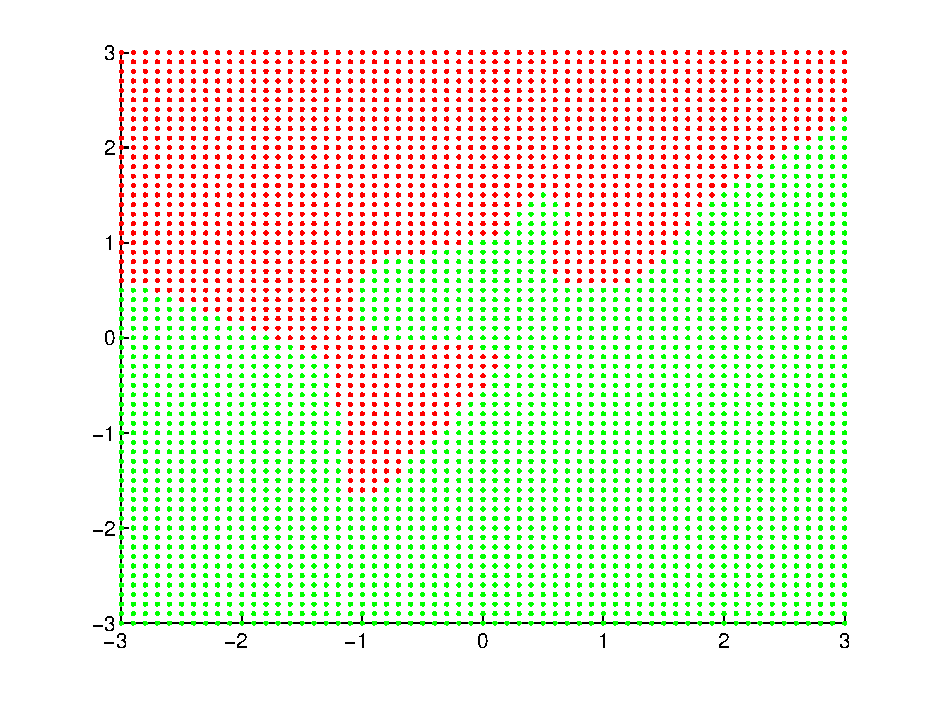
\includegraphics[width=0.6\textwidth]{./images/q31.pdf}
  \caption{The original prediktion treandt, p(c|x)}
  \label{fig:q31}
\end{figure}

\begin{figure}[!htbp]
  \centering
  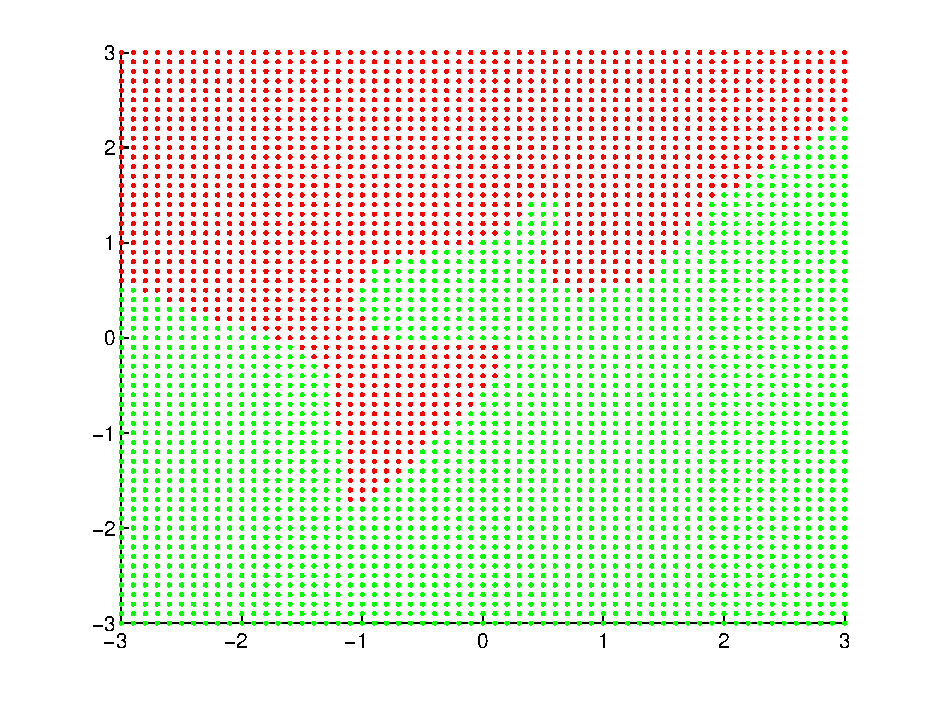
\includegraphics[width=0.6\textwidth]{./images/q32.pdf}
  \caption{the prediktion treands of the Bayes classifikation, p(x|c)}
  \label{fig:q32}
\end{figure}

As it can be seen, i figur \ref{fig:q33}, chansing the prior of one of
the classes. Makse it more or less dominent.

\begin{figure}[!htbp]
  \centering
  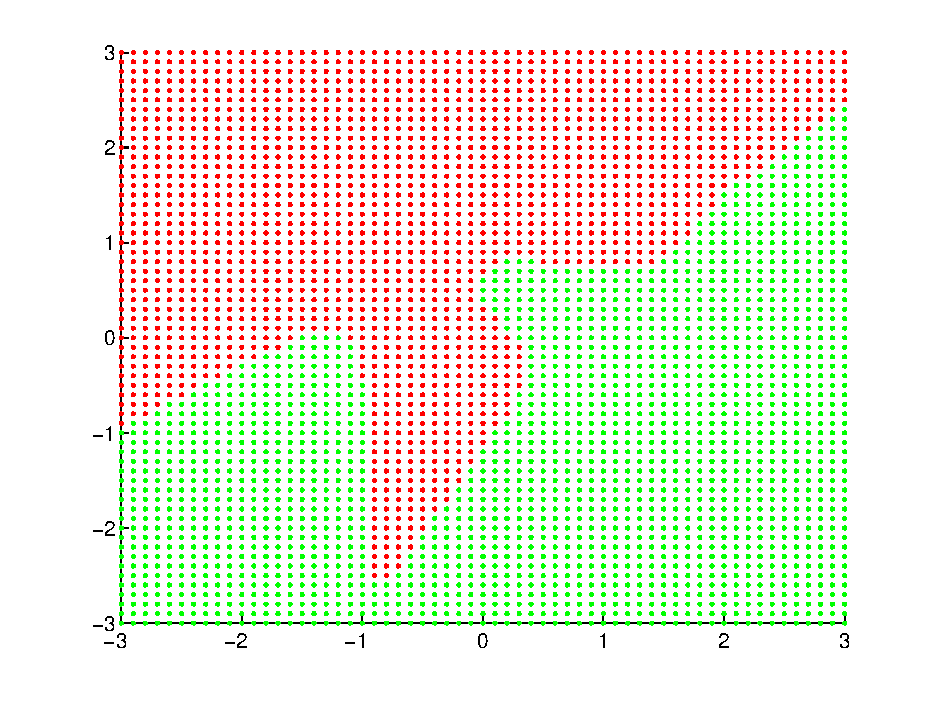
\includegraphics[width=0.6\textwidth]{./images/q33.pdf}
  \caption{the prediktion treands of the Bayes classifikation, where class one, have are prior og 1.5}
  \label{fig:q33}
\end{figure}
